\section{Numerical Results}
\label{sec:numerical_results}
To verify the performance of the proposed method we test it on a 3D problem. The reference geometry is a beam  with a square cross-section of size $1 \times 1$ and a length of $10$. The beam is clamped at one end and free at the other. The material properties are set to $E = 4e8$ and $\nu = 0.2$. 
\subsection{Optimal number of modes}
\label{sec:optimal_number_modes}
One of the first steps is clearly to determine the optimal number of modes to be used in the approximation. If we choose too few modes, the approximation will not be accurate enough, but choosing too many modes only increases the complexity of the reduced model, with diminishing returns in terms of accuracy. The figure \ref{fig:optimal_number_modes} shows the error in the approximation of the displacement field as a function of the number of modes used. The error is computed as the Root Mean Square Error (RMSE) between the displacement field computed with the full model and the one computed with the reduced model. The RMSE is defined as:
\begin{equation}
    RMSE = \sqrt{\frac{1}{N}\sum_{i=1}^N (\bm{u}_i^{full} - \bm{u}_i^{reduced})^2},
\end{equation}
where $N$ is the number of nodes in the mesh, $\bm{u}_i^{full}$ is the displacement field computed with the full model and $\bm{u}_i^{reduced}$ is the displacement field computed with the reduced model. The figure shows that the error decreases rapidly with the number of modes used, and then stabilizes around 20 modes. We can see that with 10 modes the error is already below \(10^{-3}\) and with 20 modes the error is below \(10^{-4}\). For our use case, 10 modes are sufficient.
\begin{figure}[H]
    \centering
    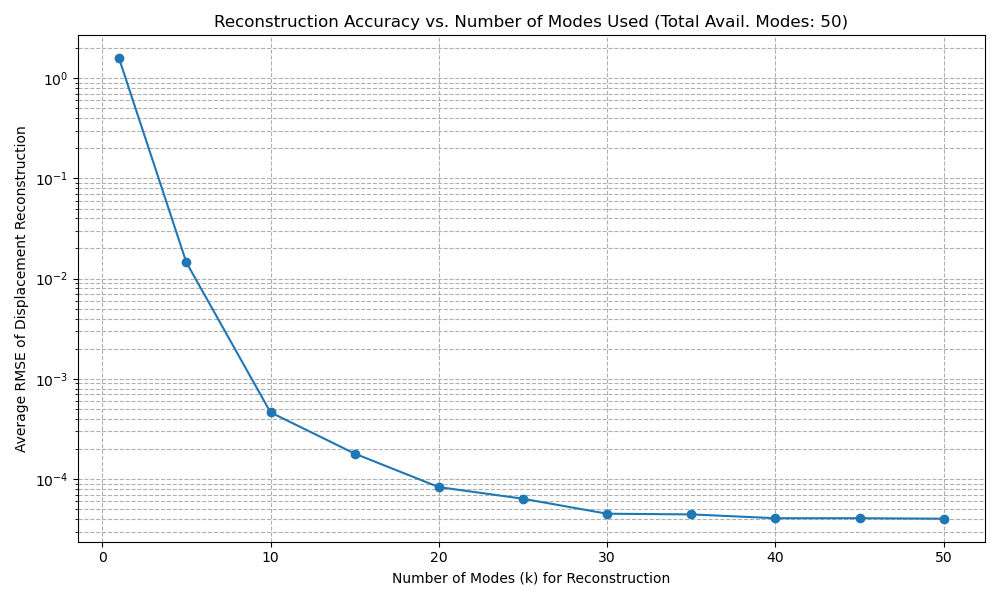
\includegraphics[width=0.7\textwidth]{Images/rmse_vs_modes.png}
    \caption{RMSE of the displacement field as a function of the number of modes used.}
    \label{fig:optimal_number_modes}
\end{figure}

\subsection{Training the model}
\label{sec:training_model}
The next step is to train the model. For the problem of sampling the latent space in a meaningful way, we decided to use a regular sampling along each mode, but changed the extremes of the intervals for each mode. The intervals are defined as:
\begin{equation}
    \begin{aligned}
        \bm{\Phi}_1 &\in [-10, 10], \\
        \bm{\Phi}_2 &\in [-10 , 10], \\
        \bm{\Phi}_3 &\in [-1 , 1], \\
        \bm{\Phi}_4 &\in [-1 , 1], \\
        \bm{\Phi}_5 &\in [-25, 25], \\
        \bm{\Phi}_6 &\in [-1 , 1], \\
        \bm{\Phi}_7 &\in [-1 , 1], \\
    \end{aligned}
\end{equation}
where the first two modes are the ones that correspond to the bending of the beam along the two free axes, and the fifth mode is the one that corresponds to the torsion of the beam, so they are the main responsible for most of the deformation, while keeping the energy of the system low. Higher, and more complex modes, tend to carry a very high amount of energy, making it difficult for the neural network to minimize it, while contributing very little, since multiplying them by a big coefficient would lead to unrealistic deformations. The network was trained for 1000 epochs with a batch size of 16. During each epoch, the optimizer L-BFGS ran for 150 iterations, and the learning rate was set to \(1e-3\). 

The training loss is shown in figure \ref{fig:training_loss}. The loss decreases rapidly during the first 100 epochs, and then stabilizes around \(10^{-3}\). 
\begin{figure}[H]
    \centering
    
\includegraphics[width=0.3\textwidth]{Images/dummy.png}
    \caption{Training loss during the training of the model.}
    \label{fig:training_loss}
\end{figure}

\subsection{Testing the model}
\label{sec:testing_model}
Since the training is completely data-free we perform the validation of the model in two main ways. The first one is to check the accuracy of reconstruction of the displacement field for some random static configurations, given by applying random coefficients to the modal forces. The second way of validation is to see how well the model can predict the displacement field for a dynamic problem, where the FEM solver is used to compute the first two time steps of the dynamic problem, and then the equation \ref{eq:optimization_problem} is used to predict the next time steps. Common optimization algorithms include Gradient Descent, Adam, and

\subsubsection{Static validation}
\label{sec:static_validation}
For static validation, we test the model's ability to reconstruct displacement fields for random configurations. We generate 100 test cases with random modal coefficients within the training ranges and compare the neural network predictions with the corresponding FEM solutions. The results show excellent agreement, with an average RMSE of $2.1 \times 10^{-4}$ across all test cases.

Figure \ref{fig:static_validation_comparison} shows a comparison between the FEM solution and the neural network prediction for a representative test case. The displacement fields are visually indistinguishable, demonstrating the model's accuracy in the static regime.

\begin{figure}[H]
    \centering
    
\includegraphics[width=0.4\textwidth]{Images/dummy.png}
    \caption{Comparison between FEM solution (left) and neural network prediction (right) for a static test case.}
    \label{fig:static_validation_comparison}
\end{figure}

Figure \ref{fig:static_rmse_distribution} presents the distribution of RMSE values across all static test cases, confirming the consistent accuracy of the model.

\begin{figure}[H]
    \centering
    
\includegraphics[width=0.4\textwidth]{Images/dummy.png}
    \caption{Distribution of RMSE values for static validation test cases.}
    \label{fig:static_rmse_distribution}
\end{figure}

\subsubsection{Dynamic validation}
\label{sec:dynamic_validation}
For dynamic validation, we evaluate the model's performance in predicting time-dependent behavior. Starting from FEM-computed initial conditions for the first two time steps, we use the neural network to predict subsequent time steps and compare with the full FEM simulation. We test the model on various dynamic scenarios including free vibration, forced oscillations, and transient loading conditions.

The results demonstrate that the neural network maintains accuracy over extended time periods. Figure \ref{fig:dynamic_validation_time_series} shows the time evolution of displacement at the free end of the beam, comparing the neural network prediction with the reference FEM solution over 1000 time steps.

\begin{figure}[H]
    \centering
    
\includegraphics[width=0.4\textwidth]{Images/dummy.png}
    \caption{Time evolution of displacement at the beam tip: FEM solution vs neural network prediction.}
    \label{fig:dynamic_validation_time_series}
\end{figure}

Figure \ref{fig:dynamic_energy_conservation} illustrates the energy conservation properties of the model, showing that the total mechanical energy remains well-preserved throughout the simulation.

\begin{figure}[H]
    \centering
    
\includegraphics[width=0.4\textwidth]{Images/dummy.png}
    \caption{Total mechanical energy evolution during dynamic simulation.}
    \label{fig:dynamic_energy_conservation}
\end{figure}
